\documentclass[fleqn]{jbook}
\usepackage{physpub}

%%%% TEXT START %%%%
\begin{document}
\begin{question}{問題1}{松井 鉄平}
次の論説を読み、設問(i)-(iv)に答えよ。(配点60点)

	Scientific understanding has probably \framebox[1cm]{(a)} more 
in the past 50 years than in all previous history. Its applications have 
made our lives \framebox[1cm]{(b)}. Increasingly,however, we recognize 
unintended \framebox[1cm]{(c)} consequences of our well-intentional activities.

	In the United Kingdom, and in Europe more generally, 
every week seems to bring a new \framebox[1cm]{(d)}, report, or debate 
on "science and society". And a good thing too. I believe we need 
to do a better job of deliberately asking what kind of world we want 
--subject to the opportunities offered by scientific advances 
and the constraints that science clarifies -- 
rather than just letting things happen. A recent \framebox[1cm]{(e)} shows 
that 84\% of Britons think that "scientists and \framebox[1cm]{(f)} make 
a valuable contribution to society" and 68\% think that 
"scientists want to make life better for the average 
person". But the real issue, as the same \framebox[1cm]{(g)} showed, 
is that roughly 50\% thought that the pace of current scientific advance 
was too fast for \framebox[1cm]{(h)} to keep up with through effective 
\framebox[1cm]{(i)} and regulation. So how best to conduct the 
dialogue, as old as democracy itself, between government 
\framebox[1cm]{(j)} and the public in 
complex scientific areas, in a way that fosters trust?

	I begin with the principles set out by the UK office of Science 
and Technology into the history 
of bovine spongiform encephalopathy$^{注1}$ : Consult widely and get 
the best people, but also make sure dissenting voices are heard 
; recognize and admit uncertainly ; and above all, 
be open and publish all advice. Try to separate risk 
assessment from risk management, and aim at management that is proportional to 
the risk involved. Whenever possible, make the facts and uncertainties 
clear and leave it to individuals to choose 
(for instance, whether to eat beef off the bone of not).

	All this is easier said than done. Even when risk can be assessed,
people's subjective views may be different (people feel that cars are 
safer than trains, even though they are more than a hundred times 
more dangerous). \underlinejpn[ア)]{そして、問題はしばしば既知の科学の枠外にあり、リスクは推測するしか仕方がない。学校、大学、クイズ番組(*1)などを通じ、確立された知識に基づき確実に答えを出せるもの、として科学をとらえている一般市民にとって、このことは特に受容しがたい。}
It is easy to say "let all voices be heard", but many will 
bring other agendas to the debate, and 
the resulting babble of voices is uncomfortable for a civil servant 
used to confidential anonymous,and consensual advice to a minister. 
However, these admitted and awkward costs 
of wide and open consultation, and of open admission of uncertainty, 
are outweighed by their trust-promoting benefits. And anyway, 
the world that deferred to authority, 
advised by confidential cabals, has gone. I do not mourn its passing.

	I see the recent UK debate and decision about extending the limited 
use of embryonic stem cells$^{注3}$ from research on human fertility$^{注4}$ 
to other specified therapeutic$^{注5}$uses as a model for the 
\underlineeng[イ)]{above principles} in action. There were three years of 
wide-ranging debate, engaging scientist, lawyers, ethicists, patient groups, 
and the general public in its many forms. Then free votes (not constrained by 
party positions in both the Lower and Upper Houses of Parliament, 
against a background of lobbying for and against; much technical information 
and misinformation; medical benefits for some; and ethical anguish for 
others. Clear decisions (by more than 2 to 1 in both houses) were made 
to allow the research to proceed, under well-specified constraints.
\underlineeng[ウ)]{This} is democracy in action, notwithstanding 
the complexity of the science.
\begin{flushright}
adapted from Science \textbf{292} 2001
\end{flushright}
\hspace*{0.5cm}
注1 : bovine spongiform encephalopathy - 牛海棉状脳症(いわゆる狂牛病) , 
注2 : クイズ番組 - quiz shows , 注3 : embryonic stem cells - はい幹細胞 , 
ES細胞 , 注4 : fertility - 不妊治療 , 注5 : therapeutic - 治療の

\begin{enumerate}
\item (a)から(j)までの空欄には、以下のどの語をいれるのが適当か、
選択せよ(同じ語が複数の欄に入ることもある)。

1) policymakers, 2) engineers, 3) poll, 4) committee, 5) better, 
6) shrinked, 7) oversight, 8)expanded, 9) worse, 10)adverse, 
11)effective, 12)government, 13)election, 14) scientists

\item 下線部 ア)を英訳せよ。

\item 下線部 イ)が指し示す'principles'とは何か、日本語で
簡潔に箇条書きせよ。

\item 下線部 ウ)の'This'の内容を、日本語1行程度で要約せよ。
\end{enumerate}
\end{question}

\begin{answer}{問題1}{松井 鉄平}
\begin{enumerate}
\item (a) 8 , (b) 5 , (c) 10 , (d) 1 , (e) 3 , (f) 2 , (g) 3 , 
(h) 12 , (i) 4 , (j) 1

\item And risk can only be assumed for the problem often lies beyond 
the framework of science. It is difficult to accept this fact, for 
ordinary people who through schools, university and quiz shows 
think of sciences as something that always have definite answers based on 
established knowledge.

\item \begin{itemize}
\item 各分野のスペシャリストを集め、意見を聴く。
\item 不確定要素の存在を認識する。
\item すべての議論を公開し、透明性を増す。
\item リスクの評価をしっかり行い、そのマネジメントを考える。
\item 不確定な部分は明確にし、できるだけ個人の判断に
任せるという仕組みを採用する。
\end{itemize}

\item 各分野の専門家が集まり、民意を反映する仕組みを通して、
ES細胞の取り扱いに関するシステムを作ったこと。
\end{enumerate}
\end{answer}

\begin{question}{問題2}{松井 鉄平}
次の説明文を読み、設問(i)-(iv)に答えよ。(配点40点)

	Time spectroscopy involves the measurement of the time relationship 
between two events. A particularly difficult problem in timing is to 
obtain a logic signal$^{注1}$ that is precisely related in time to the 
event. Some type of time pickoff circuit$^{注2}$ is employed to produce a 
logic output pulse that is consistently related in time to the beginning of 
each input of signal.

	To understand the use of timeing electronics it is important to 
understand some of the problems associated with timing. Three important 
sources of error can occur in time pickoff measurements: walk, drift, and 
jitter. Walk is the time movement of the output pulse relative to its input 
pulse, due to variations in the shape and the amplitude of the input pulse. 
Drift is the long-term timing error introduced by component aging and 
by temperature variations in the time pickoff circuitry. Jitter is 
the timing uncertainty of the pickoff signal that is caused by noise in 
the system and by statistical fluctuations of the signals from the detector.

	\underlineeng{A leading-edge method, which is the simplest means 
of deriving a time pickoff signal, produces an output logic pulse when 
the input signal crosses a fixed threshold level.} A primary disadvantage of 
this technique is that the time of occurrence of the output pulse from 
a leading-edge trigger is a function of the amplitude and rise time$^{注3}$ 
of the input signal. This time walk relationship restricts the usefulness of 
the leading-edge trigger as an accurate time pickoff device to those 
applications that involve only a very narrow range of input signal 
amplitudes and rise times.
\begin{flushright}
(adapted from EG\&G ORTEC catalog)
\end{flushright}
\hspace*{0.5cm}
注1 : logic signal - 論理回路, 注2 : time pickoff circuit - 
タイミング信号生成回路, 注3 : rise time - 立上り時間

\begin{enumerate}
\item 正確なタイミング測定で問題となる三つの要素を日本語で
簡潔に説明せよ。

\item どんな信号に対してリーディングエッジ(leading-edge)法が適用できるかを
日本で述べよ。

\item 文中の下線部を和訳せよ。

\item 次の図は'walk'を説明するための図である。図中のキーワード
($t_1$, $t_2$, V, pulse \#1, pulse \#2)をすべて用いて、'walk'を
英語5行以内で説明せよ。
\begin{figure}[htbp]
\begin{center}
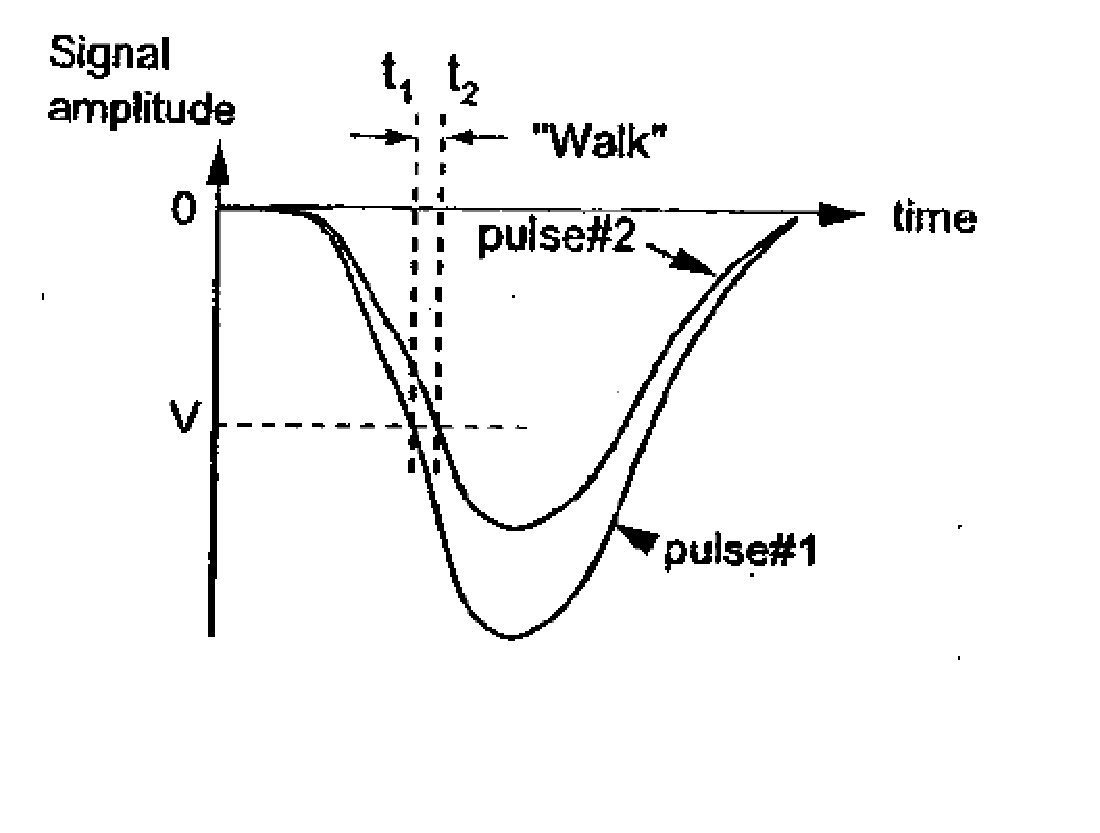
\includegraphics[width=.5\linewidth]{2002engl2.eps}
\end{center}
\end{figure}

\end{enumerate}
\end{question}

\begin{answer}{問題2}{松井 鉄平}
\begin{enumerate}
\item \begin{itemize}
\item walk - input pulse の形状や振幅のばらつきを測定器が
時間の違いだと認識してしまうこと。

\item drift - 部品の老朽化、pick off circuitの熱的なばらつきによる
(長期で表れる)タイミングエラー
 
\item jitter - システムのノイズと測定器の統計誤差が原因となる
pick off signal のタイミング不確定性
\end{itemize}

\item input signalの振幅、立上り時間のrangeが狭いもの

\item 一番単純なタイミング生成回路の原理であるリーディングエッジ方では、
input signalがあるthreshold levelを横切る時にoutput logic pulseが
生成される仕組みになっている。

\item In this graph the time pick off circuit recognizes pulse \#1 at $t_1$, 
when it crosses V. Pulse \#2 on the other hand is recognized at $t_2$, 
by the same reason. Even though two pulses occured at the same time, 
the circuit counts pulse \#2 after pulse \#1. This difference or movement in 
time is called ``walk''.

\end{enumerate}
\end{answer}
\end{document}
